\section{Comparing Transfers via Sun-Earth Staging Orbits to Direct Transfers}\label{sec:StagingComparison}
Just like the example tradespace provided in \cref{sec:Transfers} with \cref{fig:tradespace}, for a
given cislunar departure orbit, the direct transfers are compared to the staging orbit ones. The
tradespaces for all of the cislunar departure orbits utilized in this investigation are provided in
\cref{chap:Tradespaces}, along with figures illustrating the departure orbits themselves, but some
are introduced in this section to facilitate the comparison. In general, for the scenarios examined
in this investigation, transfers with lower times-of-flight tend to have higher maneuver costs and
vice versa. As demonstrated in the example of \cref{fig:tradespace}, the transfer points lie mostly
in the upper-left and bottom-right sections of the tradespace. In all of the tradespaces computed
in this investigation, the blue points representing the direct transfers mostly lie to the left of
the red staging orbit transfers but well above the modified Hohmann transfer baseline,
corresponding to direct transfers with lower TOF but much higher $\Delta v$ compared to the staging
orbit transfers. However, there are often some transfers in the tradespace where the $\Delta v$
lies below the baseline of the modified Hohmann transfer and even below those of the staging orbit
transfers. The tradeoff between time-of-flight and maneuver cost highlights the importance of
mission-specific priorities when selecting a transfer strategy.


\subsection{A Simple Cost Function}
In the example of \cref{fig:tradespace}, the transfer family that directly departs the system
contains both the minimum-TOF and minimum-$\Delta v$ solutions. In the provided case, the
minimum-$\Delta v$ solution of the direct transfers has a lower TOF than most of the staging orbit
transfers. However, this is not always the case, as demonstrated by \cref{fig:lowDeltav}. Here,
while the direct transfers still have a lower TOF, the staging orbit transfer family reaches a
lower $\Delta v$. As a result, often a transfer selection needs to be made balancing TOF and
maneuver cost. A cost function helps select desirable transfers that balance the two parameters.

\begin{figure}[H]
    \centering
    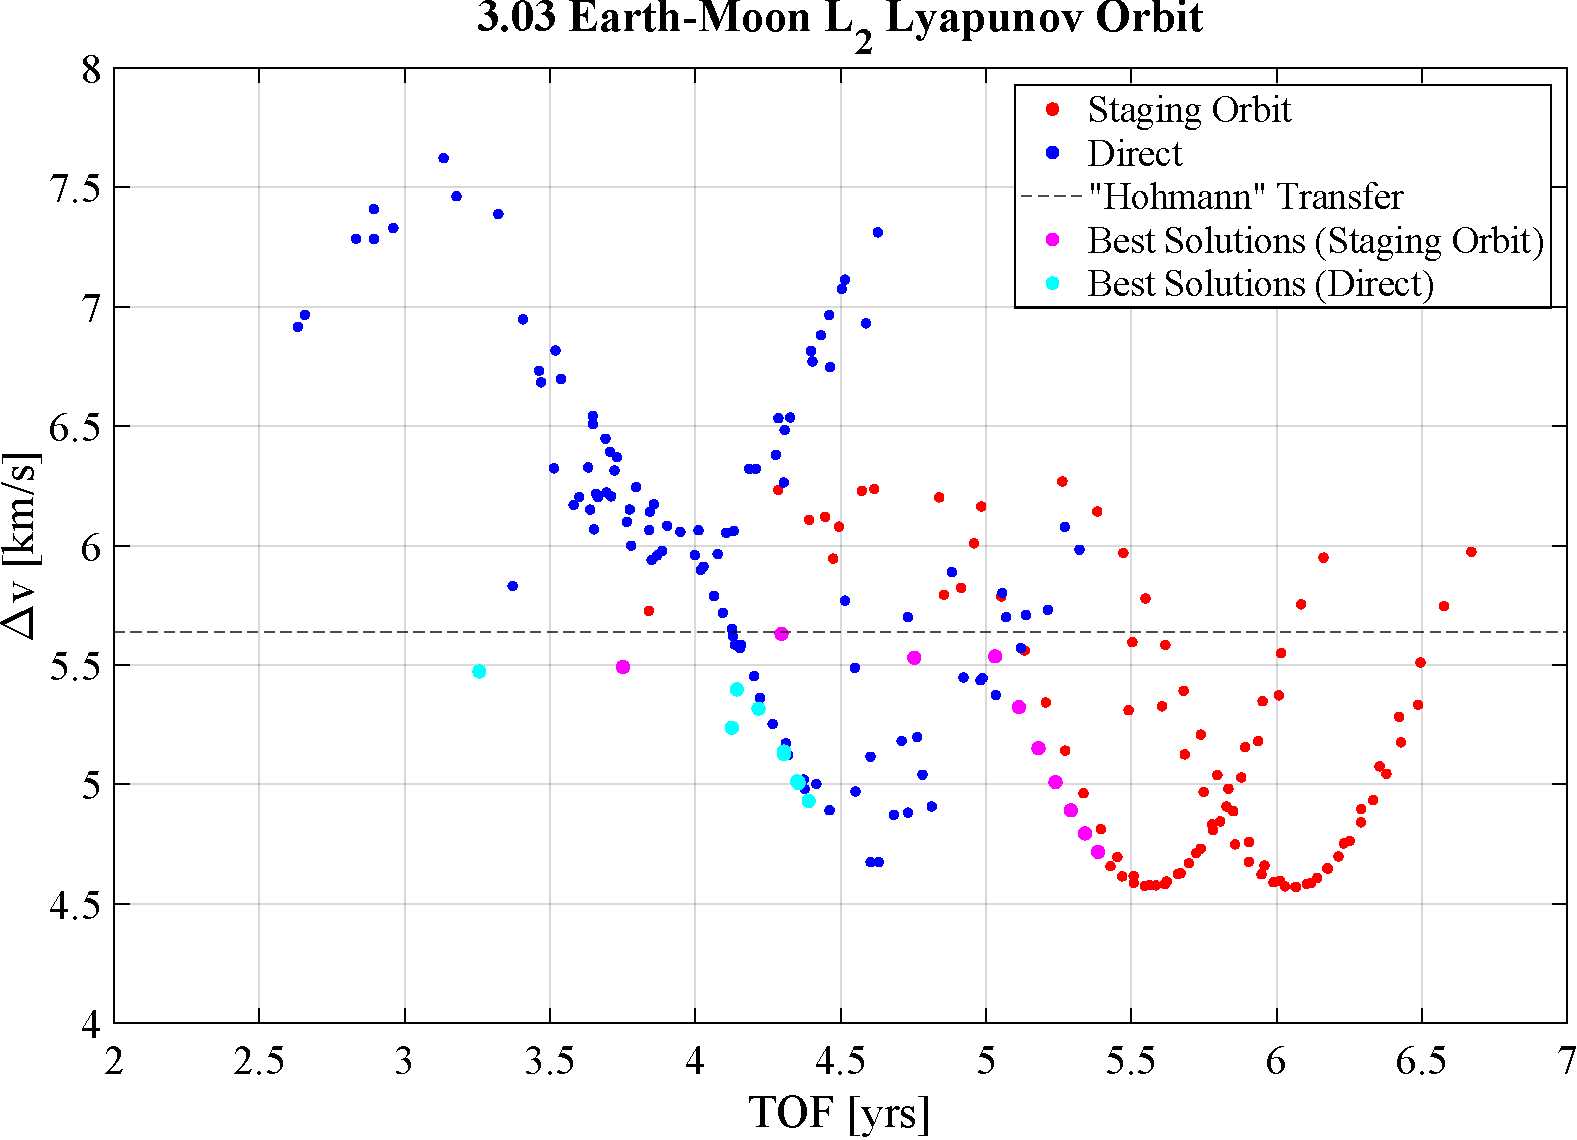
\includegraphics[width=0.75\textwidth]{figures/TradeSpace_L2Lyapunov_3_03.pdf}
    \caption{Transfer tradespace departing from an Earth-Moon $L_{2}$ Lyapunov orbit ($JC=3.03$).}
    \label{fig:lowDeltav}
\end{figure}

If total TOF and total maneuver $\Delta v$ are considered to have units of years and km/s,
respectively, then the values have similar orders of magnitude for the computed transfers.
Consequently, an appropriate cost function places weights on the two parameters according to the
desired transfer characteristics for a given mission:
\begin{equation}
    J=\alpha TOF+\beta\Delta v,
    \label{eq:costfunction}
\end{equation}
where $J$ is the cost function value and $\alpha$ and $\beta$ are design variables for adjusting
the cost function. $\alpha$ and $\beta$ can be adjusted to place higher priority on TOF or
$\Delta v$, depending on the particular application. This investigation utilizes values of
$\alpha=5$ and $\beta=2$ as a representative cost function to prioritize lowering the TOF while
still looking for decreased maneuver costs. The cost function is applied to transfers in the
tradespace that are below the modified Hohmann transfer $\Delta v$ baseline, and the ten transfers
that have the lowest $J$-value from each transfer category are determined to be the lowest-cost
transfers for the selected application. In \cref{fig:lowDeltav}, there are cyan points for the
direct transfers and magenta ones for the staging orbit transfers. The cost function provides a
systematic approach to identify transfers that balance time-of-flight and maneuver costs, ensuring
that the selection aligns with mission priorities and operational constraints.

\subsection{Comparing Lowest-Cost Solutions between Transfer Types}
Comparing the lowest-cost solutions highlights the differences between direct transfers and staging
orbit transfers, with direct options generally achieving shorter times-of-flight at slightly higher
or comparable maneuver costs. In \cref{fig:lowDeltav}, among the lowest-cost solutions selected
with the cost function, the direct options have a lower average TOF than the staging orbit ones,
$4.04$ and $4.94$ years, respectively, while the transfers with staging orbits achieve a slightly
lower average $\Delta v$ cost, $5.207$ km/s compared to $5.238$. The earlier example from
\cref{fig:tradespace}, now including the lowest-cost solutions from the cost function in
\cref{fig:costTradespace}, produces similar results. In contrast, the direct options in
\cref{fig:lowBoth} have both lower times-of-flight and maneuver costs when compared to the staging
orbit transfers, $4.33$ years and $4.869$ km/s average for direct transfers versus $4.82$ years and
$5.148$ km/s for those with a staging orbit. In all of the tradespaces computed in this
investigation, the lowest-cost direct solutions perform better than the lowest-cost staging orbit
transfers with regards to TOF. While the lowest-cost staging orbit solutions often have slightly
lower $\Delta v$ costs on average, the significantly longer times-of-flight outweigh those
benefits, and there are still many cases where the direct options require lower maneuver costs.

\begin{figure}[H]
    \centering
    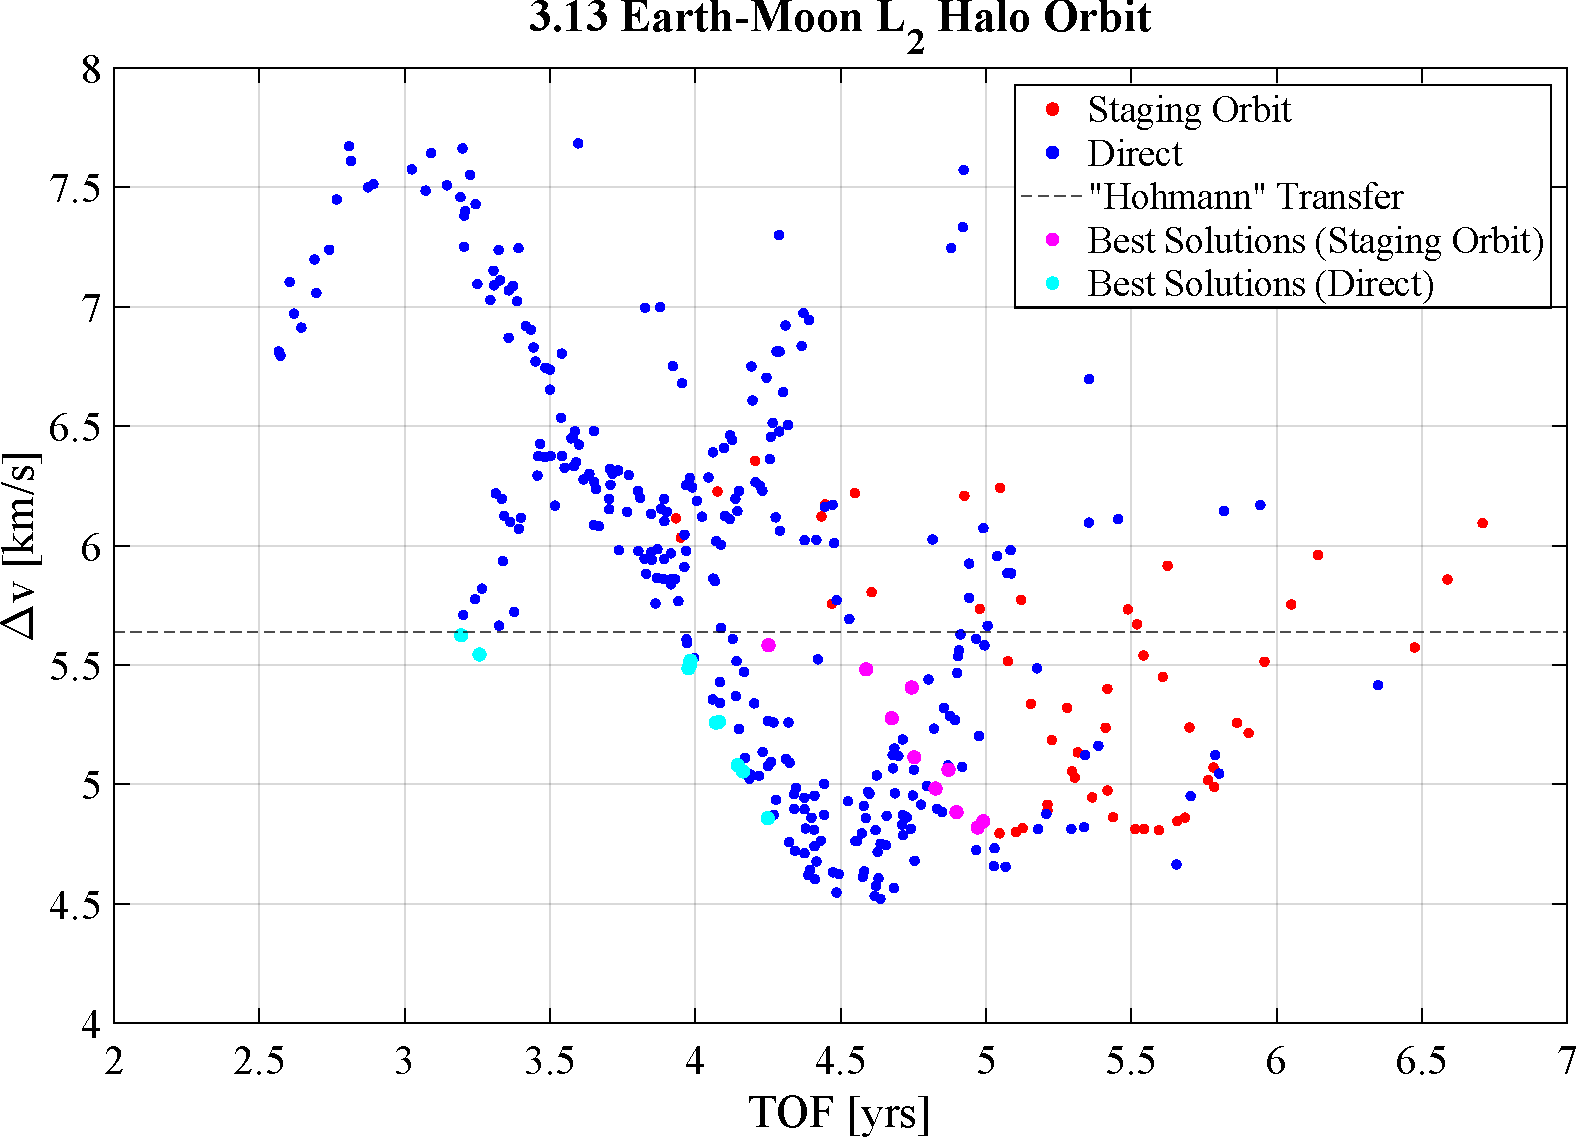
\includegraphics[width=0.75\textwidth]{figures/TradeSpace_L2Halo_3_13.pdf}
    \caption{Transfer tradespace departing from an Earth-Moon $L_{2}$ northern halo orbit ($JC=3.13$).}
    \label{fig:costTradespace}
\end{figure}

One downside to the direct departure method is that it relies on the spread and rapid departure of
the Earth-Moon unstable manifolds arcs. A major contributing factor is the proximity of the
cislunar orbit to the Moon or Earth. If manifold arcs crash into one of the primaries or get
captured by their gravitational effects, it delays the departure of the arcs from the system and
also impacts their distribution in position space, leading to fewer available transfers. The
stability of the orbit also plays a role in affecting the departure time since orbits with higher
instability have manifolds that depart the orbit vicinity faster. When there are fewer departure
arcs available, it leads to fewer successful end-to-end transfers with direct departures,
demonstrated in \cref{fig:fewDirect}. Note that there is a significantly decreased number of
available direct solutions and that the ones that do exist no longer follow a familial pattern as
in the previous examples. Since the staging orbit transfers only require one manifold arc to
interface with the Sun-Earth orbit stable manifold, there is still a full range of staging orbit
transfers available. However, the lowest-cost direct solutions still outperform the staging orbit
ones here.

\begin{figure}[H]
    \centering
    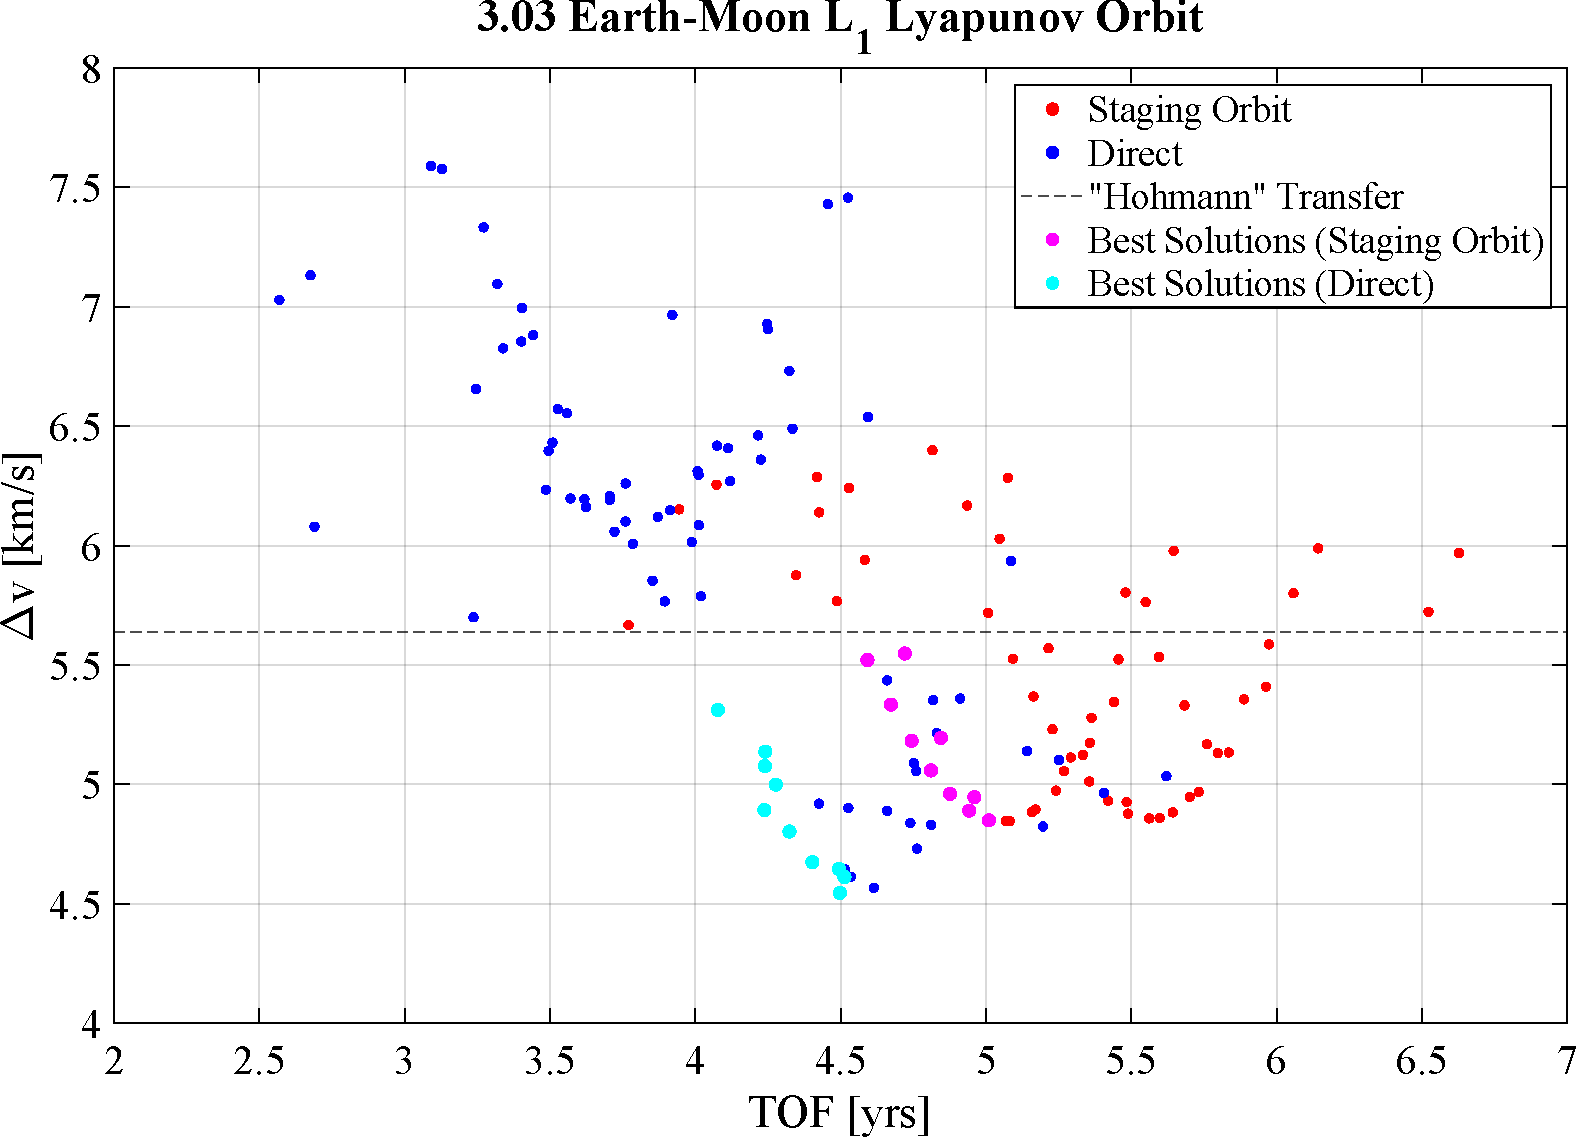
\includegraphics[width=0.75\textwidth]{figures/TradeSpace_L1Lyapunov_3_03.pdf}
    \caption{Transfer tradespace departing from an Earth-Moon $L_{1}$ Lyapunov orbit ($JC=3.03$).}
    \label{fig:lowBoth}
\end{figure}

The results of this investigation and the provided observations demonstrate that the methodology
developed to construct end-to-end cislunar-to-Mars transfers that directly depart the Sun-Earth
system performs better overall than the strategy that incorporates an intermediate Sun-Earth halo
staging orbit. The lowest-cost solutions that directly depart the cislunar orbits utilized in this
investigation always have a faster average TOF than the lowest-cost staging orbit transfers. While
the direct options only sometimes have a lower $\Delta v$ maneuver cost than the staging orbit
ones, the decrease in TOF is significant enough to outweigh the potential slight increases in
maneuver cost. The findings highlight the efficiency and practicality of direct transfer options
for mission planning, particularly when the minimization of TOF is a critical mission objective.

\begin{figure}[H]
    \centering
    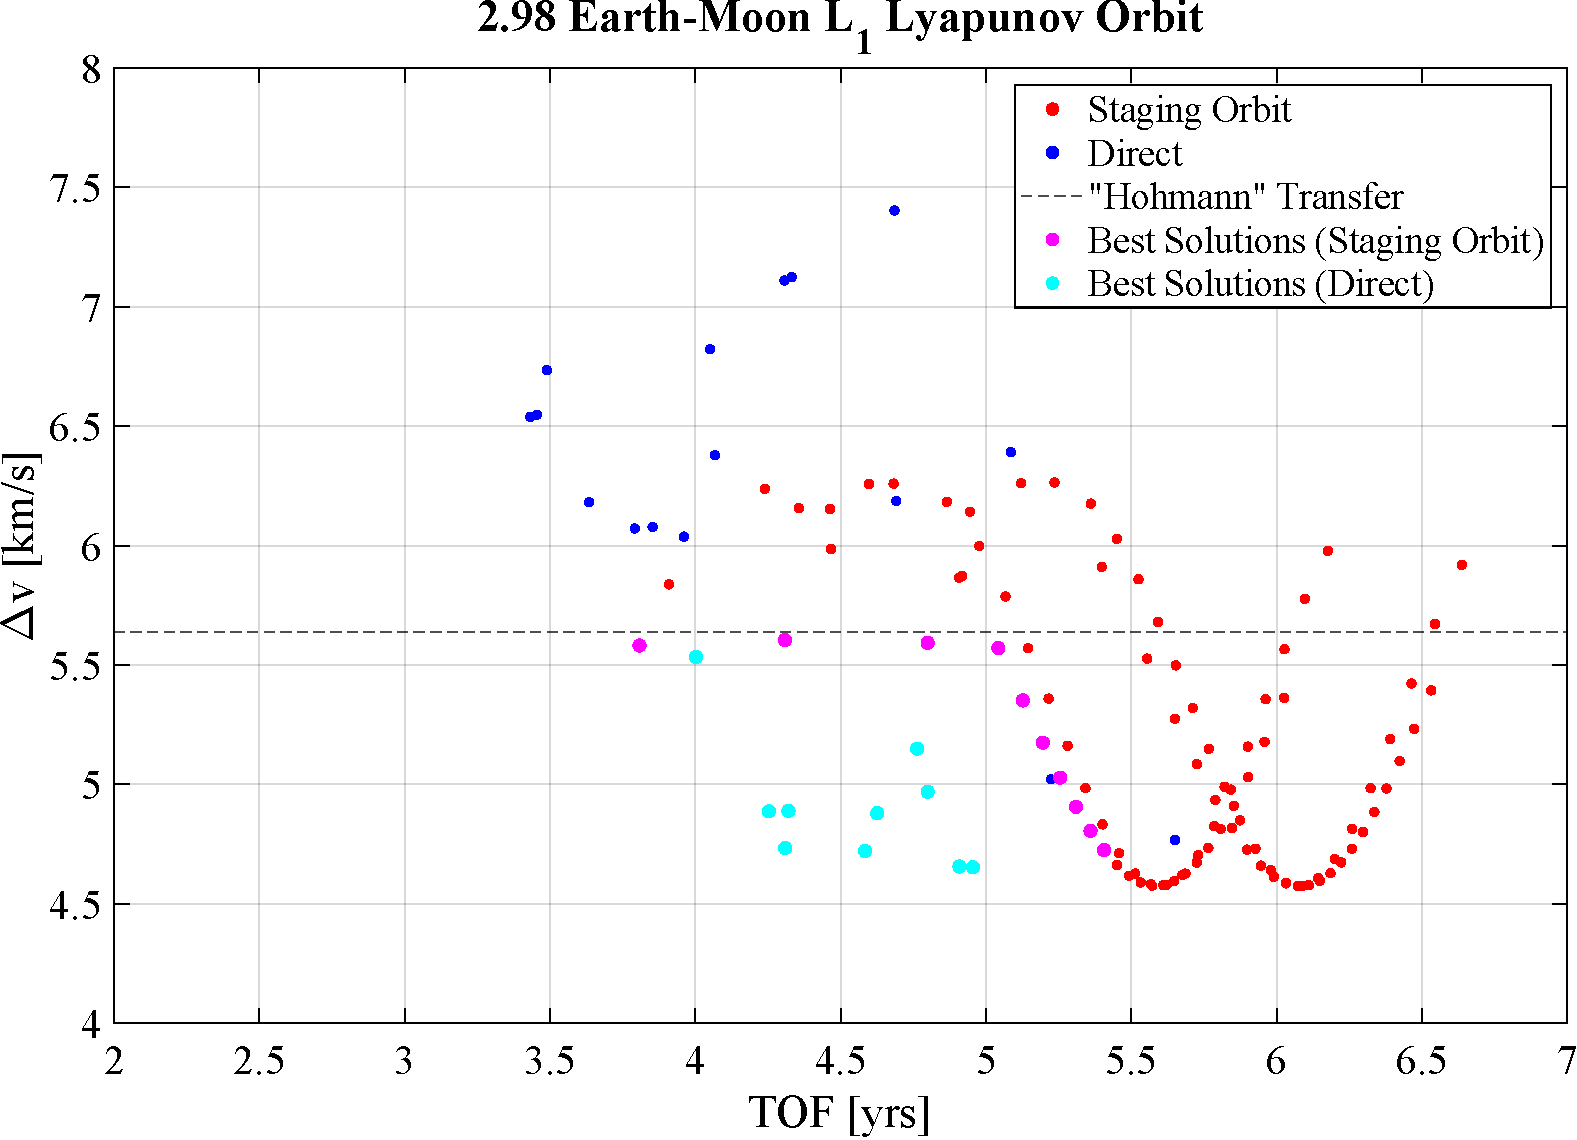
\includegraphics[width=0.75\textwidth]{figures/TradeSpace_L1Lyapunov_2_98.pdf}
    \caption{Transfer tradespace departing from an Earth-Moon $L_{1}$ Lyapunov orbit ($JC=2.98$).}
    \label{fig:fewDirect}
\end{figure}
